\section{Conclusions}
\label{sec:conclusions}

\begin{figure*}
  \centering
  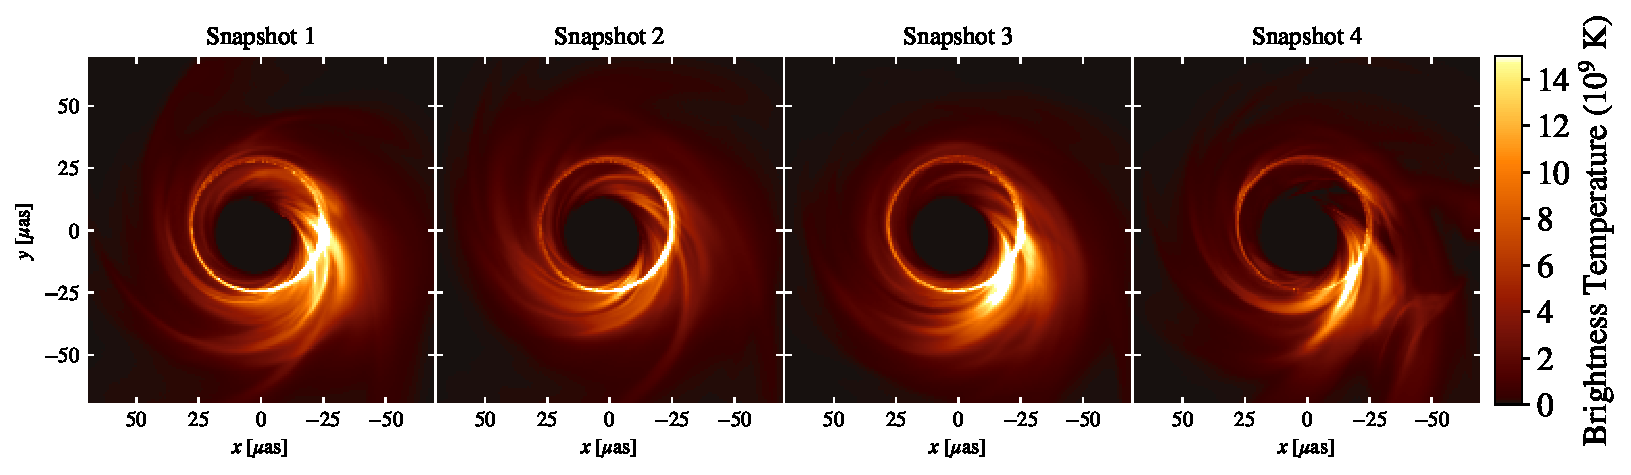
\includegraphics[width=\textwidth]{figures/bestbet_imgs_frames.pdf}
  \caption{%
    230\GHz full resolution snapshots from a fiducial model in the
    best-bet region.
    This model passes 10/11 constraints.
    The different panels are snapshots taken from the ``best time'',
    when the synthetic observation has good \uv coverage.%
  }
  \label{fig:bestbet_imgs_snapshot}
\end{figure*}

\begin{figure*}
  \centering
  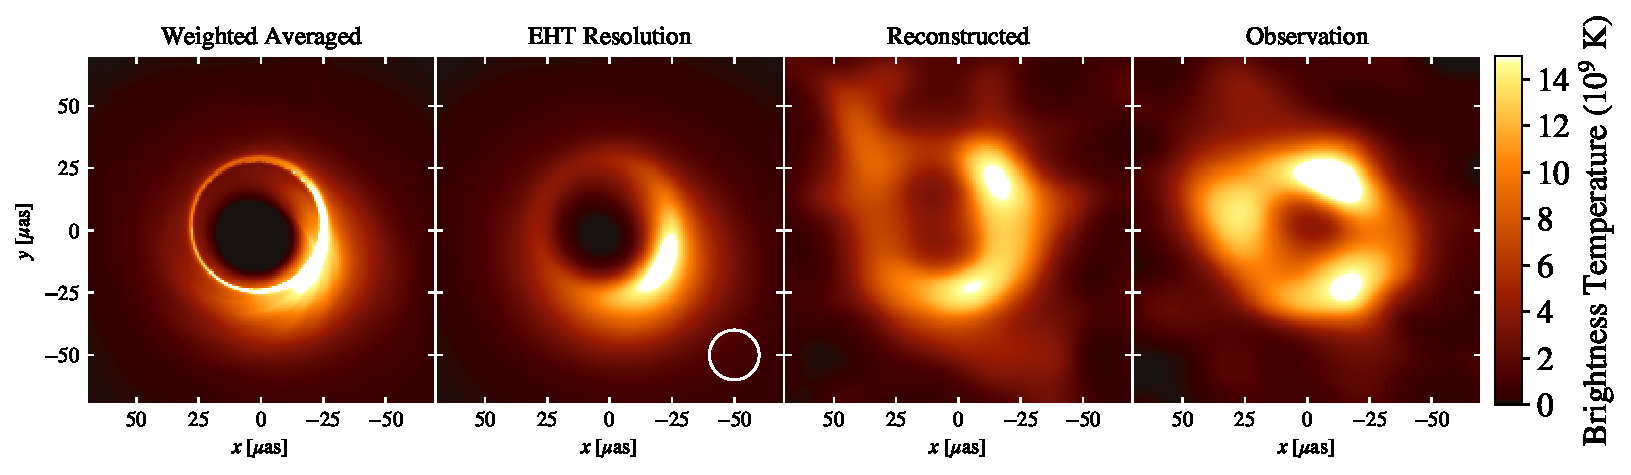
\includegraphics[width=\textwidth]{figures/bestbet_imgs_allframes.pdf}
  \caption{%
    Reconstructions of a fiducial model in the best-bet region,
    compared to the April~7 observation.
    This is the same model shown in
    Figure~\ref{fig:bestbet_imgs_snapshot}.
    The leftmost panel shows an average of the snapshots used in the
    synthetic observation, weighted by the number of baselines at
    each time.
    The second panel shows the averaged image convolved with a 20\uas
    beam, which roughly approximate EHT resolution.
    The third panel shows an average image reconstructed from
    synthetic data using the fiducial model.
    The final image shows the average image reconstructed from April~7
    EHT data.%
  }
  \label{fig:bestbet_imgs}
\end{figure*}

We have made a first comparison of the EHT 2017 \sgra data to a state-of-the-art library of ideal general relativistic magnetohydrodynamics (GRMHD) models.
The models assume that the mass and distance to \sgra are known and that the central object is a black hole described by the Kerr metric.
We use multiple simulation pipelines and find that for a given model configuration, independent simulations are remarkably consistent (Appendix~\ref{app:numerical}).

The model parameters are: whether the horizon magnetic field is strong or weak (MAD or SANE, respectively); the black hole spin $\abh$; and the inclination angle $i$ between the line of sight and the accretion flow orbital angular momentum vector.
The electron distribution function (eDF) also has one or more parameters.
In our ``fiducial'' model set, run with three independent codes, the eDF is determined using the so-called $\Rh$ prescription (Section \ref{sec:models}).
We have also considered exploratory models with alternate eDF prescriptions and alternate initial conditions.

We have selected and applied 11 heterogeneous observational constraints.
Six derive directly from EHT VLBI data, two derive from 86\GHz VLBI observations with the GMVA, one from variability of the 230\GHz light curve, and one each from the 2.2\um flux density and the X-ray luminosity.

Five structural constraints derive from EHT VLBI data.
When combined these constraints reject about 75\% of our fiducial models.
The EHT cut favors $\abh \ge 0$ and avoids edge-on ($i = 90\degree$) models and models with equal ion and electron temperatures ($\Rh = 1$).
We are {\em not} able to constrain the source position angle due to sparse baseline coverage.
The 2017 EHT observations are, nevertheless, quite constraining.  New EHT observations with additional antennas will be even more constraining.

The strongest EHT-derived constraint is \mring width.  The physical interpretation of \mring fits is challenging because fitting is done after the model is observed with limited baseline coverage and limited temporal sampling.  Nevertheless, some interpretation is possible.  For example, there is a trend toward lower width at higher inclination that eliminates many of the edge-on models. This can be understood since many edge-on models have higher peak brightness temperature than face-on models due to Doppler boosting of emission from the approaching side of the disk. The flux density, which must average 2.4Jy, is approximately proportional to the solid angle of the source multiplied by a typical brightness temperature, so when brightness temperature is higher, solid angle must be smaller.  If the source is a ring of fixed radius, then, higher brightness temperature implies a narrower ring.

Four constraints derive from non-EHT data that are contemporaneous or near-contemporaneous.
Combined, the non-EHT constraints reject 94\% of fiducial models.
The non-EHT cut favors strongly magnetized (MAD) models and eliminates most models at $i > 50\degree$ \citep[consistent with interpretations of GRAVITY results][]{2020A&A...643A..56G}, and also eliminates all models with equal ion and electron temperatures.
These results highlight the value of continued multiwavelength monitoring of \sgra.

The non-EHT constraints, like the EHT-derived constraints, exhibit  complicated but interpretable trends across parameter space. A full discussion of fiducial model trends will be explored in later papers, but as an example consider the 86GHz size constraint.  At $\Rh = 1$, the mean 86GHz FWHM of SANE models {\em decreases} as inclination increases.  The origin of this trend is very similar to the origin of the trend in \mring width with inclination.  At $\Rh = 1$ the electrons are hot and the source is optically thin. The peak brightness temperature of edge-on models is higher than that of face-on models due to Doppler boosting of emission from the approaching side of the disk, and thus at fixed flux density the source becomes smaller as inclination increases.  At $\Rh = 160$, by contrast, the trend is reversed and the mean 86GHz FWHM of SANE models {\em increases} as inclination increases.  In $\Rh = 160$ SANE models the electrons are cool in the disk midplane and most emission arises along the walls of the jet (see Figure 4 of \M87PaperV).  The equatorial plane is relatively opaque and Doppler-boosted emission is hidden. In face-on models one is looking down the jet and the source appears relatively small; in edge-on models the jet is extended perpendicular to the line of sight and the source appears larger.  Interestingly, MAD models exhibit only weak trends in 86GHz size with inclination, in part because MAD models are more optically thin than SANE models and also because MAD models are more slowly rotating than SANE models, weakening Doppler boosting.

\sgra is variable, but is not as variable as we expected based on our fiducial models.
We have used two tests to compare the variability of models and data.
One characterizes variability in the 230\GHz light curve (including simultaneous ALMA data) and the other characterizes structural variability expressed through fluctuations in the visibility amplitudes.
The light curve variability is the tightest of all 11 constraints: it rejects 95\% of our fiducial models.
We find that strongly magnetized (MAD) models are more variable than weakly magnetized (SANE) models and, grouped together, both SANE and MAD models are more variable than the data.
The structural variability constraint measures the slope and amplitude of the power spectrum of the VA variability.
Remarkably, we find that the power spectrum slope is consistent for all models, while the power spectrum amplitude is consistent for 43\% of fiducial models.

%cmf addressing referee comment 1 (Not sure where to place this, first version)

The higher variability of the MAD models compared to the SANE models is a consequence of the quasi-regular magnetic flux expulsion events that are a defining feature of the MAD models. Magnetic flux through the horizon builds up until it exceeds a threshold, and then escapes over a few dynamical times through the surrounding accretion flow.  As flux is escaping, strongly magnetized low density regions push aside plasma in the region close to the black hole that produces most of the 230GHz emission and this produces large fluctuations in the 230GHz flux density.  The SANE models, by contrast, exhibit relatively steady accretion through the equatorial plane.

%The difference in variability between the fiducial MAD and SANE models could be understood by stronger variations in the accretion rate for MAD models. The MAD models exhibit large, irregular fluctuations in the %quasi-periodic oscillation
%mass accretion rate, with changes up to a factor of 10 \citep[see, e.g.][]{2021arXiv211102518F} between low and high accretion states. These changes in the mass accretion rate are connected to variations in the absorptivity and emissivities introducing fluctuations in the observed 230\,GHz light curves. On the other hand the SANE models do not generate strong oscillations in the mass accretion rate. In general this behaviour is almost independent of the electron distribution function and the inclination. However, a more detailed study of the connection between the mass accretion rate and the radiative properties is required.

%Next we turn to the 86,\GHz size. To understand the variation in the 86\,GHz size between the MAD and the SANE models we need to take into account that in the MAD case the emission is mainly generated in the midplane whereas in the SANE case the emission is spread over a larger region. As such the 86\,GHz size of the MAD models is nearly independent of the choice of the $R_{\rm high}$ parameter and inclination. In the SANE case the emission is shifted towards the jet with increasing $R_{\rm high}$ values and together with the increased Doppler boosting with inclination and black hole spin leads to larger 86\,GHz images not in agreement with the observations.

%Lastly, we provide a explanation for the differences between MAD and SANE models in the case of the 2.2\um flux. The MAD models are hotter than the SANE models (see Fig. \ref{}) generation higher 2.2\um fluxes. Since the thermal emissivities behave like $\exp{-R_{\rm high}^2/3}$ the drop in the 2.2\um fluxes with $R_{\rm high}$ can be understood. Similar to the 86\,GHz source the 2.2\um flux increase with inclination and spin due the enhanced Doppler boosting.}


The failure of nearly all fiducial models to match the light curve variability is interesting.
It may signal the presence of extended, slowly varying structure that is resolved out by EHT, or it may signal that future models need to incorporate collisionless effects (potentially modeled as viscosity and conductivity) or a more sophisticated treatment of electron thermodynamics including cooling. In addition, different initial geometries and polarities of the magnetic field could lead to more slowly varying structures \citep{2021arXiv211103689N}. If when combined these effects were to reduce \mi{3} by 30\% then many MAD models would be consistent with the data.

None of the fiducial models survive the full gauntlet of 11 constraints.
If we set aside both variability constraints, however, then there 2 fiducial models that pass the remaining 9 constraints in all simulation pipelines (a few more survive in one model set but not the other).
These models in the ``best-bet region'' are strongly magnetized (MAD) and have $\Rh = 160$, positive spin, and low inclination, with ($\abh, i$) = (0.5, 30\degree) and (0.94, 30\degree).
They have accretion rates $\dot{M} = (5.2$--$9.5)\times 10^{-9}\msun\yr^{-1}$, which are consistent with earlier estimates and overlap with accretion rates in wind-fed models, $\sim 10^{-8} \msun\yr^{-1}$ \citep{2020ApJ...896L...6R}.
The $\abh = 0.5$ MAD with $i=30\degree$ model is presented in Figure~\ref{fig:bestbet_imgs_snapshot} as snapshots and in Figure~\ref{fig:bestbet_imgs} as a weighted average, a convolved average, and a reconstructed average image from synthetic data.
One of the reconstructed average images from the 2017 EHT observations is shown in the rightmost panel in Figure~\ref{fig:bestbet_imgs} for comparison.

We produced synthetic SEDs, and therefore bolometric luminosities $L_\mathrm{bol}$, for all fiducial models.
Typically $L_\mathrm{bol}$ is dominated by a synchrotron bump in the submm and for the best-bet region is $(6.8$--$9.8)\times10^{35}\ergps$; the corresponding radiative efficiency $L_\mathrm{bol}/(\dot{M} c^2)$ is $(1.3$--$3.0)\times 10^{-3}$.
The maximum radiative efficiency over the entire fiducial model set is 0.08 (for a MAD, $\abh = 0.94$, $\Rh = 1$ model), which is necessary but not sufficient to justify our neglect of radiative cooling in the GRMHD evolution.

All our fiducial models produce bipolar outflows, and for each we measured the outflow power $P_\mathrm{out}$, defined in Section~\ref{sec:discussions}.
Consistent with earlier work we find that outflow power is higher for strongly magnetized (MAD) models than for comparable weakly magnetized (SANE) models, and increases by more than an order of magnitude from $\abh = 0$ to $|\abh| = 0.94$.
For models in the best-bet region, $P_\mathrm{out} = (1.3$--$4.8) \times 10^{38}\ergps$, corresponding to an outflow efficiency $P_\mathrm{out} /(\dot{M} c^2)$ of 0.25--1.6.
Such large outflow efficiency is only possible if energy is extracted from a spinning black hole via the mechanism proposed by  \cite{1977MNRAS.179..433B}.
It is an open question how these powerful outflows might interact with incoming gas in a self-consistent accretion model that follows plasma over a larger range in radius than our fiducial models.
It is also an open question whether the outflow power could be detected in the dense but crowded galactic center environment.
Notice that this outflow luminosity is comparable to the spindown luminosity of the Crab pulsar.

All fiducial models assume a particular parameterization for the electron distribution function (the $\Rh$ prescription), use a common initial setup (a magnetized torus), and assume the black hole spin vector and torus orbital angular momentum are aligned or anti-aligned.
To partially control for the errors introduced by these assumptions we have included a set of exploratory models.  These include several eDF prescriptions, a wind-fed model that tracks accretion from stellar winds down to the scale of the horizon, and tilted disk models in which the black hole spin and torus angular momentum are misaligned.

Our non-thermal models are remarkably similar to their thermal counterparts.
For the limited set of non-thermal eDF prescriptions we consider here the 230\GHz image structure differs very little for models in which the non-thermal electrons are introduced mainly in the jet.  The 230\GHz variability is not detectably different than corresponding thermal models.\footnote{The non-thermal models are imaged over $5\times 10^3\tg$, so constraints on $\mi{3}$ are weaker than for the fiducial models, which are imaged for 3 times as long.}
The 86\GHz size and flux density, which are the most restrictive non-EHT constraints, are not detectably affected by the addition of non-thermal electrons for most non-thermal models (except $\kappa = 5$ models).
Nonthermal electrons consistently increase the 2.2\um flux density over similar thermal models, however.
Accelerating even a small fraction of the electron population into a non-thermal tail risks overproducing 2.2\um emission.
The 2.2\um (and submm through mid-IR) flux density therefore provides the strongest eDF constraints.
Future EHT analyses would benefit from incorporating submm constraints \citep[e.g.,][]{2019ApJ...881L...2B} and, because model submm SEDs are highly variable, the submm and 2.2\um data should be as close to simultaneous as possible.

The stellar wind-fed models of \citet{2020ApJ...896L...6R} feature the best-motivated treatment of boundary and initial conditions for \sgra models.
They differ from our torus-initialized fiducial models in that they follow plasma from its ejection from stars on known orbits down to the event horizon.
We have imaged these models using an $\Rh$ prescription for the electron temperature, with $\Rh$ adjusted in the otherwise parameter-free models to produce the correct time-averaged 230\GHz flux density.
The two models considered here, both with $\abh = 0$, fail the 86\GHz flux, \mring width, and $\mi{3}$ constraints.
This does {\em not} imply that wind fed models are ruled out; they clearly merit further investigation with longer integrations over a broader range of eDFs and $\abh$.

In general, black hole accretion flows can be tilted in the sense that the orbital angular momentum of the disk and the spin angular momentum of the hole are misaligned.
Tilted disks have not until now been included in EHT analyses because
\emph{i}) it is conceivable that accretion flows align either by consistently oriented long term accretion or by some analog of the Bardeen-Petterson effect \citep{1975ApJ...195L..65B}; and
\emph{ii}) the tilted disk parameter space is larger than the aligned disk parameter space by two dimensions: the tilt angle and the longitude of the observer.
We considered models with tilt $30\degree$ and $60\degree$, observed at a single longitude.
The integrations were too short ($\no{3000}\,\tg$) to provide strong constraints on tilt, but we find that the \mring width test is particularly sensitive to tilt and rejects a progressively larger fraction of the models as tilt increases at the single observing longitude studied here.
Tilted models clearly merit further investigation.

Our fiducial models and variable $\kappa$ non-thermal models have been run with independent GRMHD codes and imaged with independent radiative transfer codes.
The outcomes are largely consistent (see Appendix~\ref{app:numerical} for details).
The code comparisons were valuable and helped identify multiple issues in the independent simulation sets.
The consistency between codes is remarkable given the complexity of the modeling process and the scope for error.
Tracking down the remaining discrepancies (for example, in the 2.2\um flux density) and developing a quantitative error budget is an essential but difficult task for the future.
